\chapter{Methodology}
\label{cp:methodology}

\section{Apparatus}\label{sec:apparatus}

In this experiment, we calibrated the Omega pressure transducer in the Iowa State University wind tunnel laboratory. \autoref{fig: IMG_3131.jpeg}.

\begin{figure}[htpb]
    \centering
    \includegraphics[width=0.75\linewidth]{Figures/IMG_3131.jpeg}
    \caption[Photograph of the Omega pressure transducer]{Photograph of the Omega pressure transducer}
    \label{fig: IMG_3131.jpeg}
\end{figure}

In \autoref{fig: IMG_3131.jpeg}, we connected the tubing to two ports on the Omega pressure transducer. The first port served as the main port, receiving the total pressure, while the second port was the reference pressure port. The Omega pressure transducer then outputted the dynamic pressure by calculating the difference between the main and reference ports.

\begin{figure}[htpb]
    \centering
    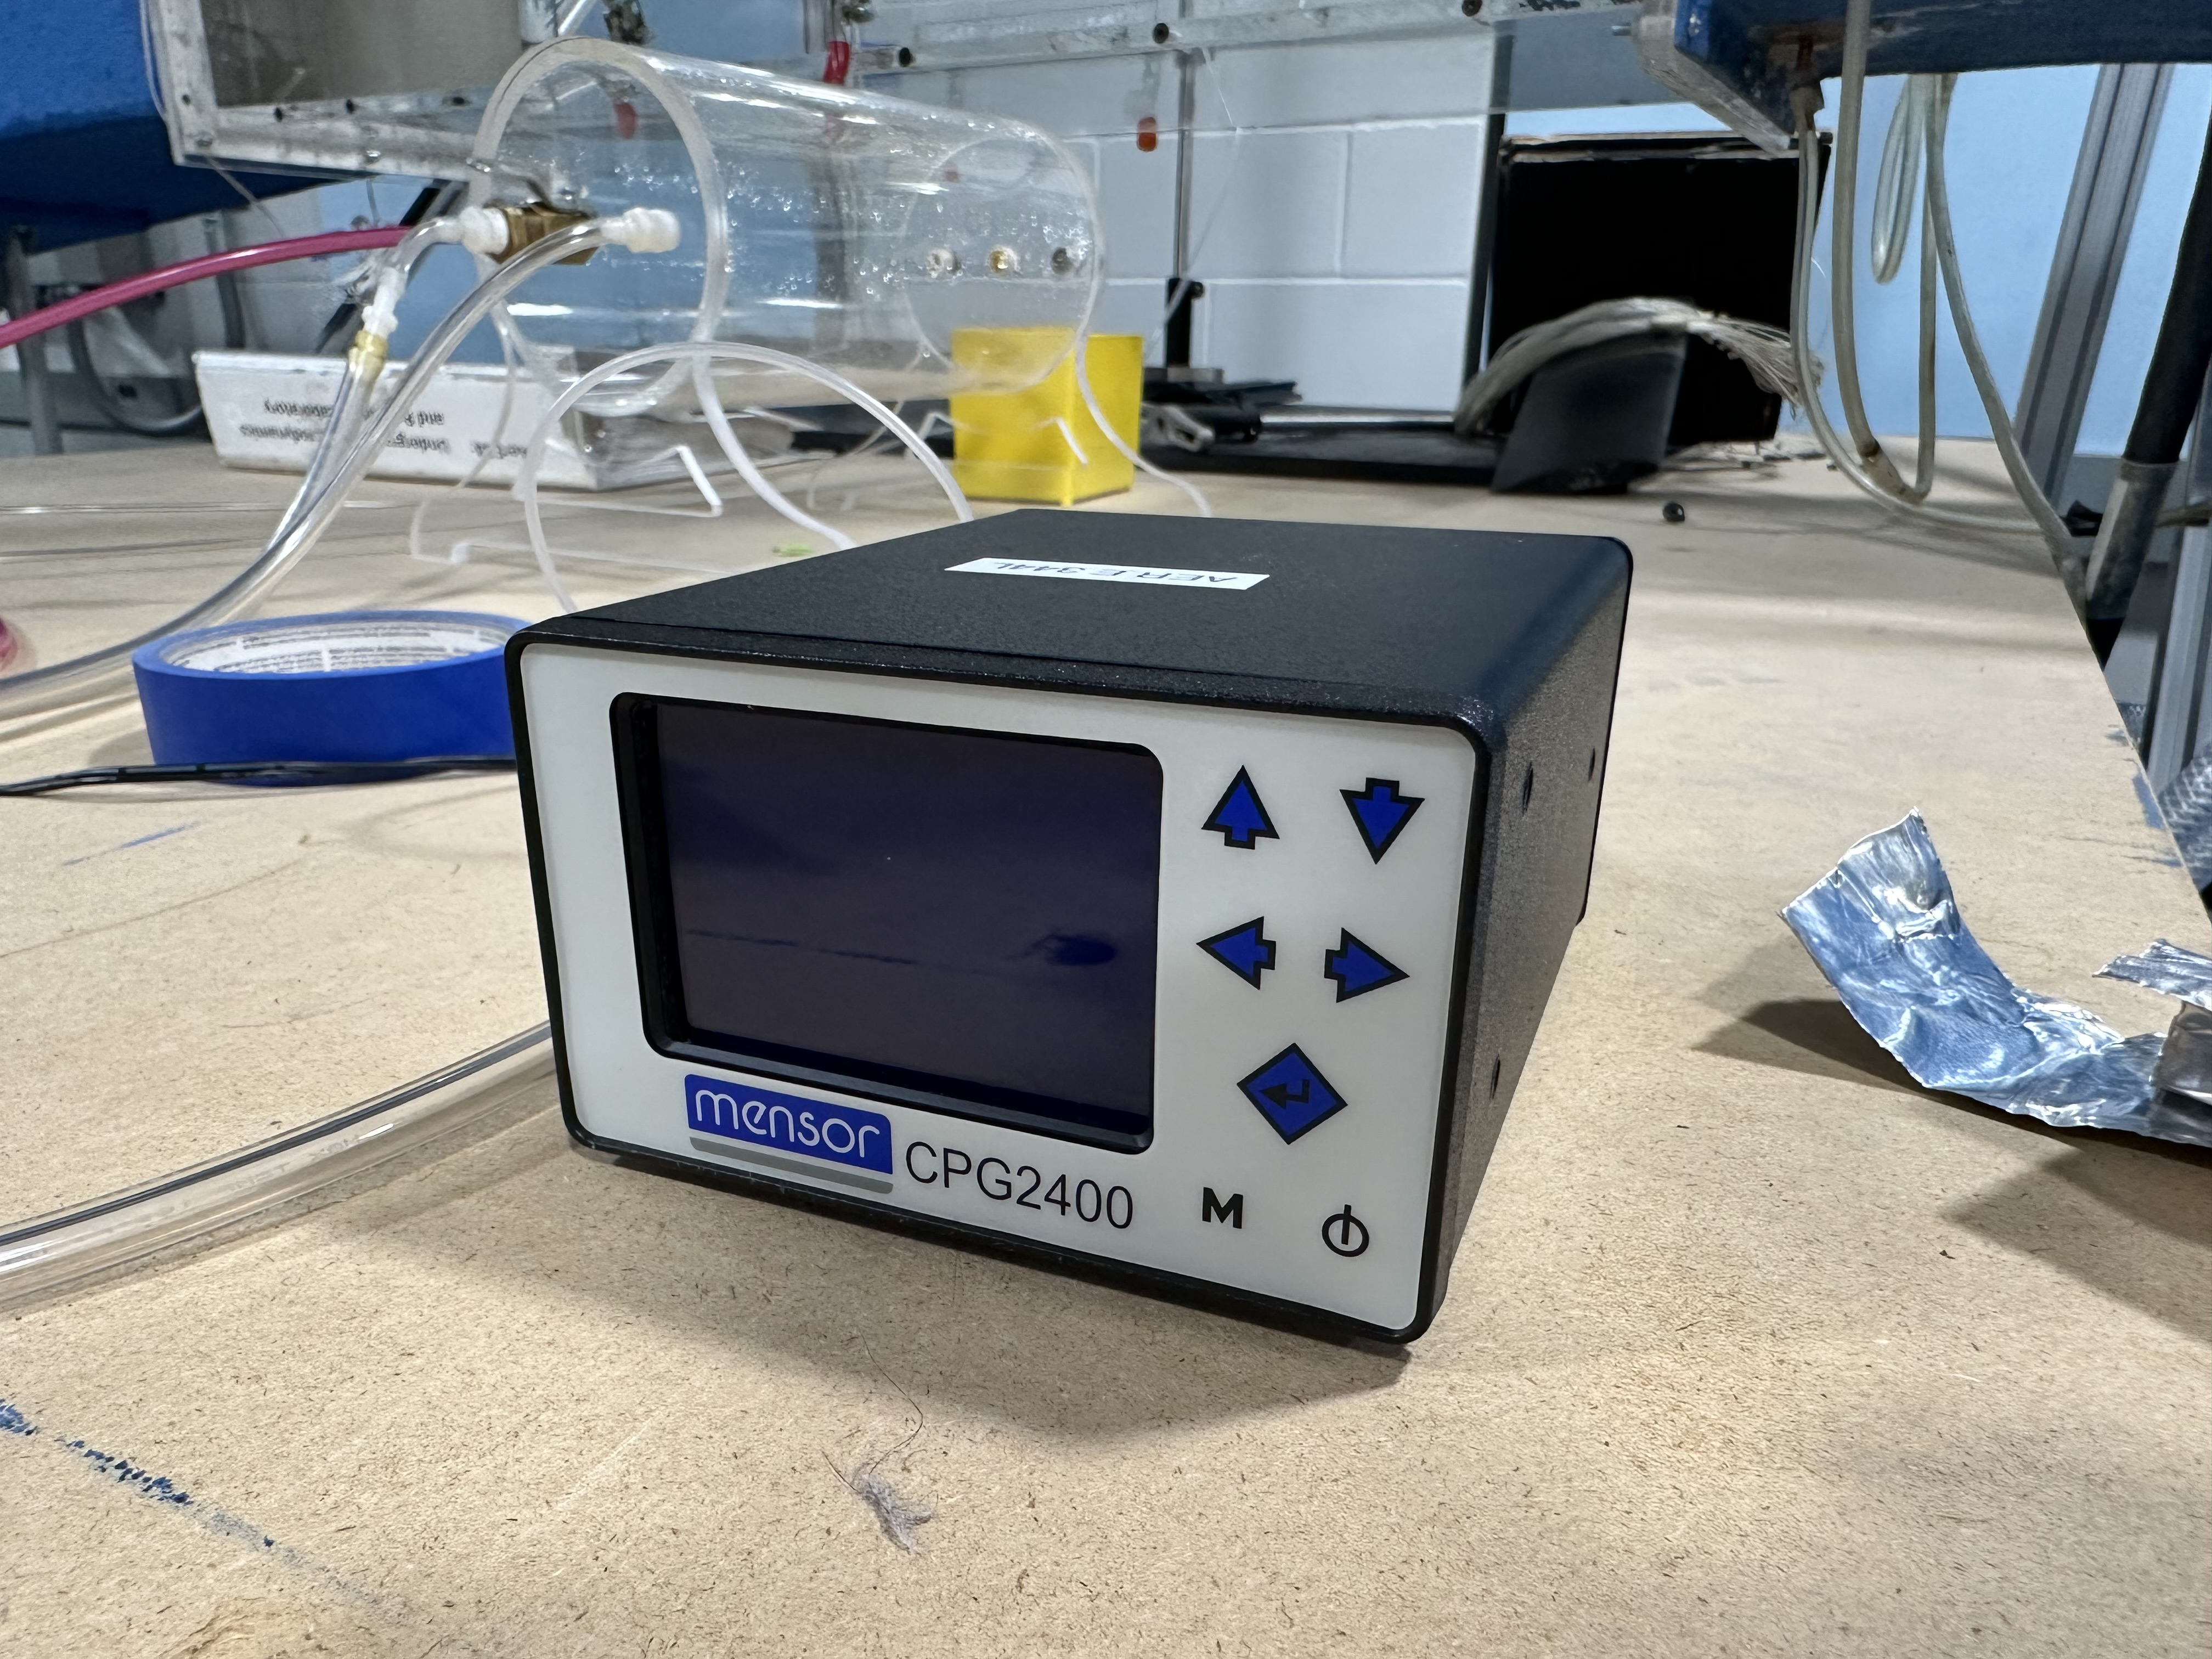
\includegraphics[width=0.75\linewidth]{Figures/IMG_3130.jpeg}
    \caption[Photograph of the Mensor Digital Pressure Gauge]{Photograph of the Mensor Digital Pressure Gauge}
    \label{fig: IMG_3130.jpeg}
\end{figure}

\begin{figure}[htpb]
    \centering
    \includegraphics[width=0.75\linewidth]{Figures/IMG_3129.jpeg}
    \caption[Photograph of the setup that we used to calibrate the Setra electronic manometer]{Photograph of the setup that we used to calibrate the Setra electronic manometer}
    \label{fig: IMG_3129.jpeg}
\end{figure}

\begin{figure}[htpb]
    \centering
    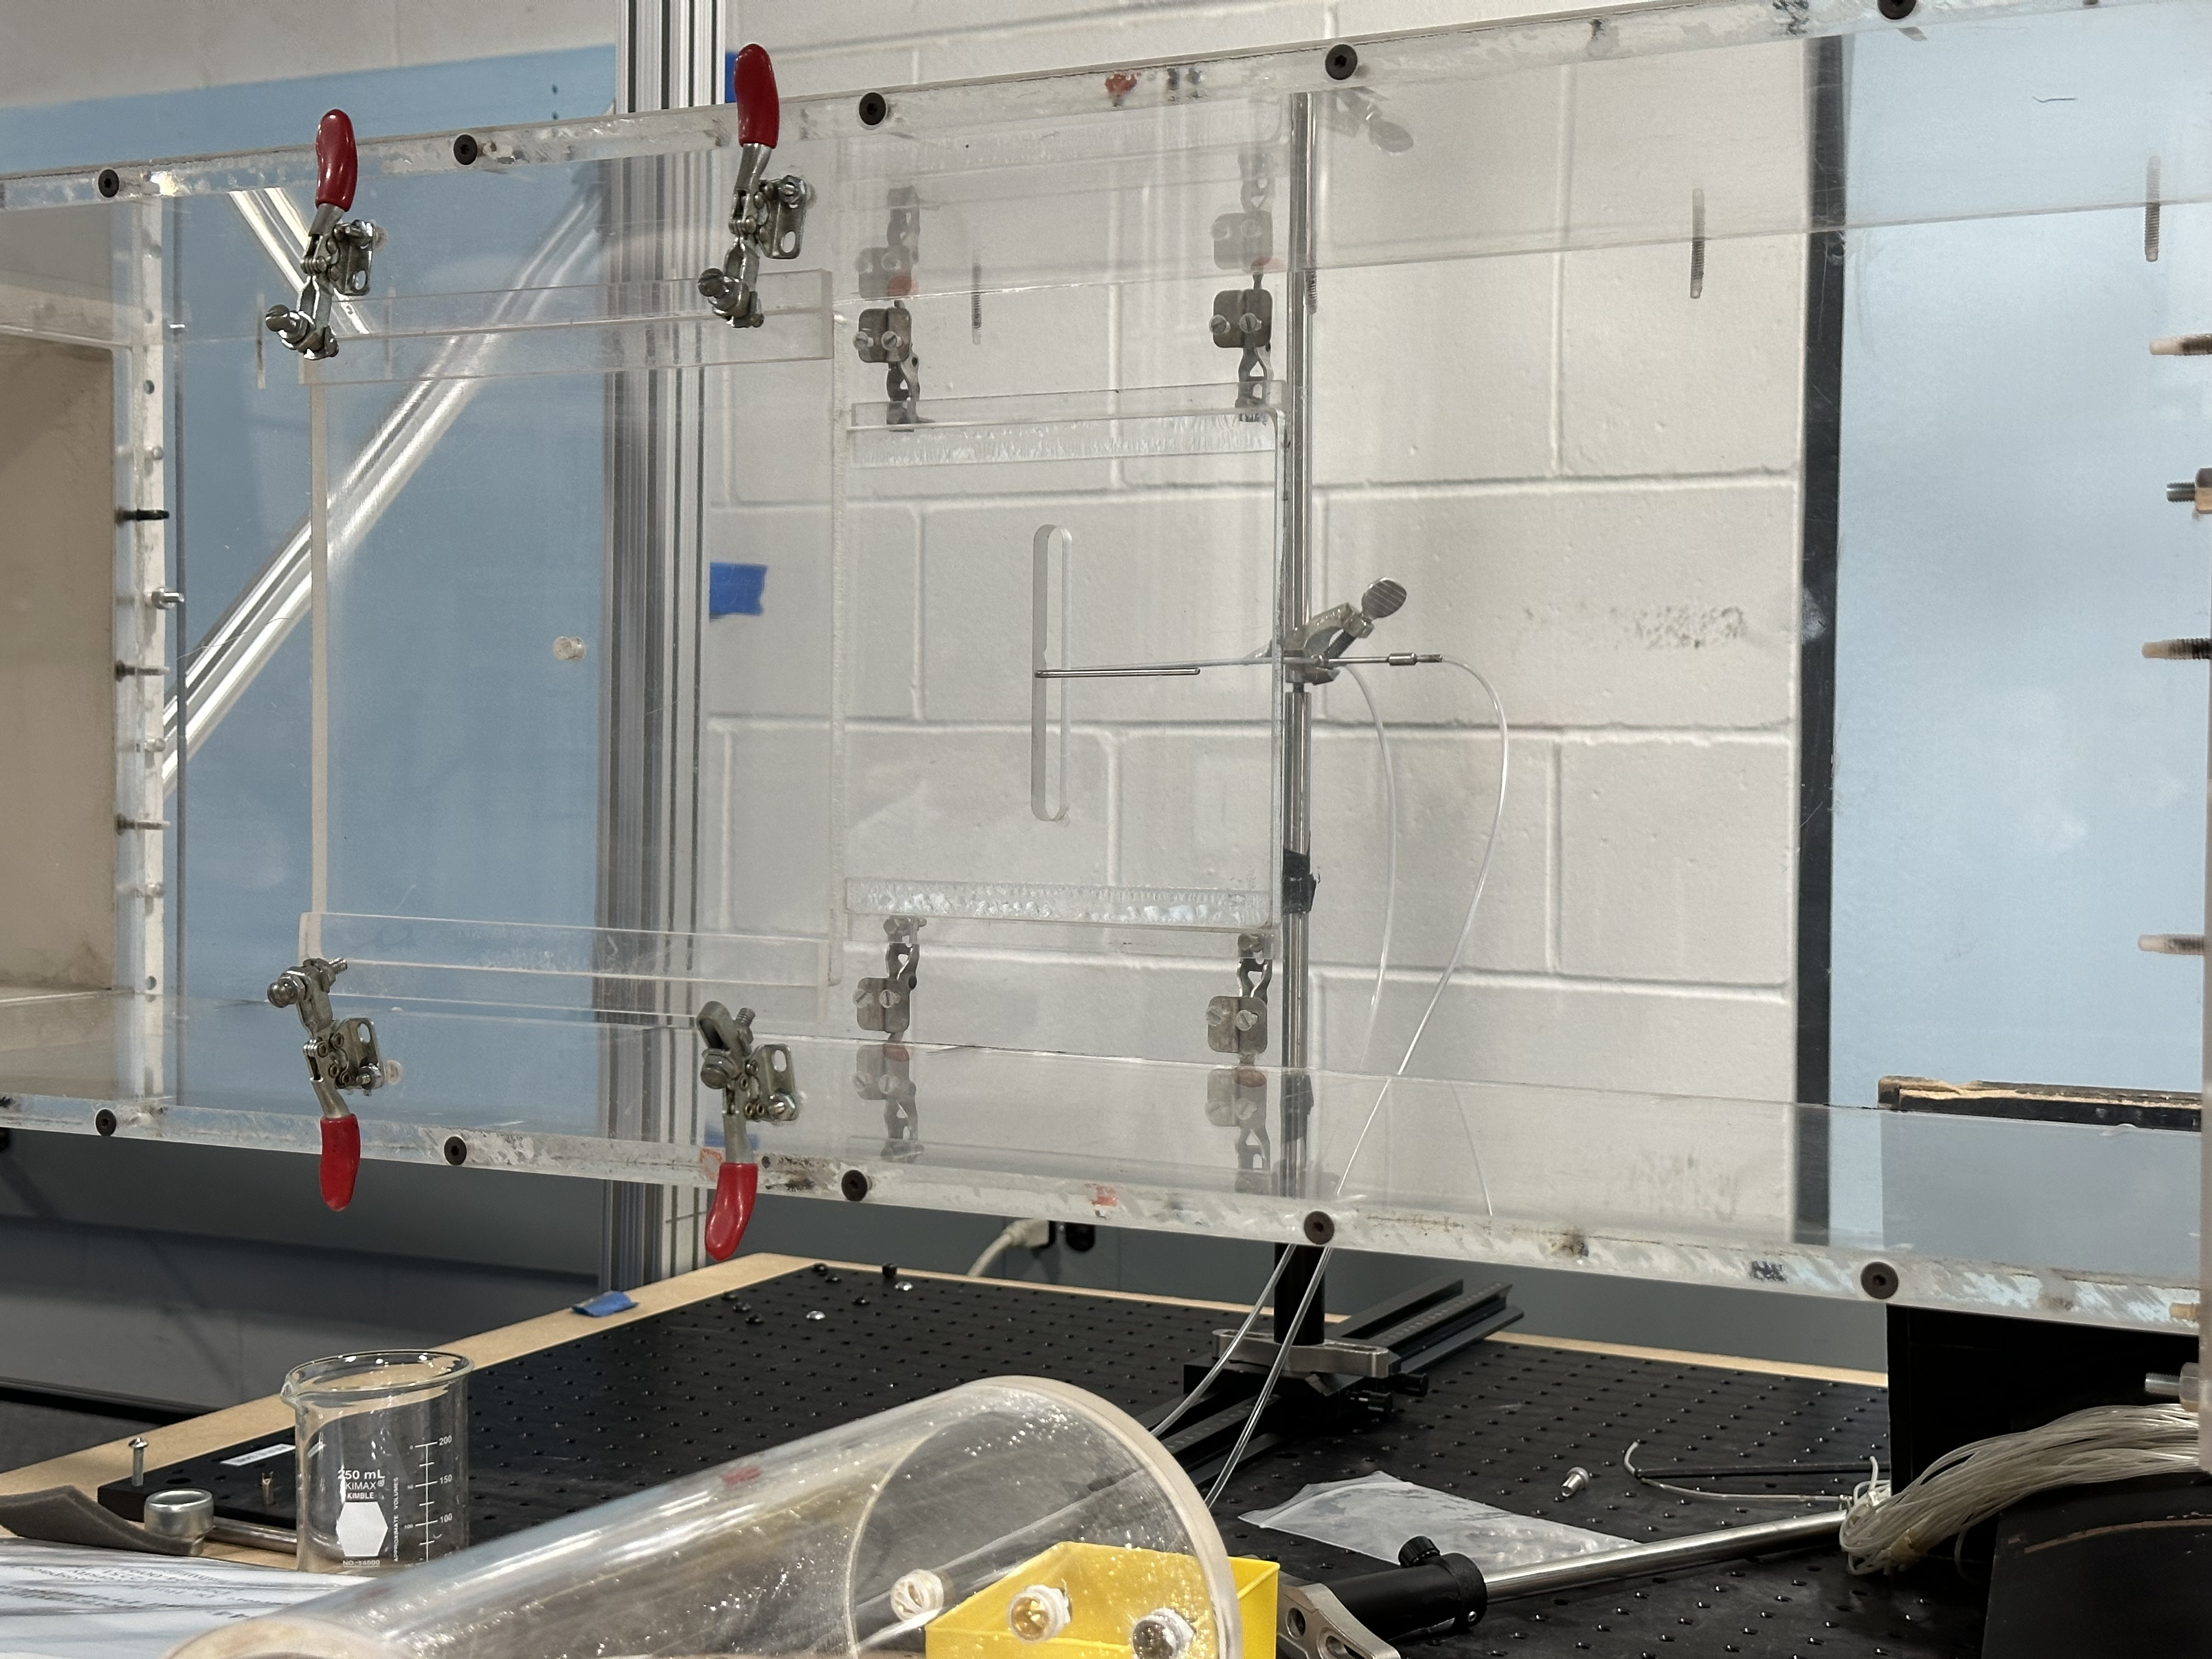
\includegraphics[width=0.75\linewidth]{Figures/IMG_3132.jpeg}
    \caption[Photograph of the pitot tube that we used in the second part of the lab.]{Photograph of the pitot tube that we used in the second part of the lab.}
    \label{fig: IMG_3132.jpeg}
\end{figure}



\newpage

\section{Procedures}\label{sec:procedures}

\subsection{Electronic Manometer Calibration}\label{sec:calibration}

\underline{Apparatus:} Tubes are connected from the Mensor Digital Pressure Gauge to the plenum chamber and from the Setra electronic manometer to the plenum chamber. The pump is connected to the valve on the plenum chamber. \\
\underline{Procedure:} 
\begin{enumerate}
    \item Measure the voltage with 0 pressure in the chamber. 
    \item Pressurize close to 5 in H20 and record the voltage. 
    \item Open the chamber valve and release about 0.5 in H20 of pressure.  
    \item Wait for the pressure to stabilize and record the voltage.  
    \item Repeat steps 3-4 until the pressure is 0. Take at least 10 data points. If you reach 0 pressure before you have 10 data points, re-pressurize to 5 inH20 and repeat the process until you have acquired enough data.
\end{enumerate}

\subsection{Wind Tunnel Dynamic Pressure Distribution Mapping}\label{subsec:dynamic_pressure_mapping}

\underline{Apparatus:} The pitot tube is connected to the Setra electronic manometer. The total pressure tube of the test section is connected to the main port on the electronic manometer and the static pressure tube is connected to the reference port of the manometer. \\
\underline{Procedure:}
\begin{enumerate}
    \item Set the wind tunnel to 10 m/s. 
    \item Start the pitot tube at the wall and sample the voltage from the electronic manometer. Save the file. 
    \item Move the pitot tube in from the wall 1 cm. and sample the voltage from the electronic manometer. Save the file.  
    \item Repeat for step 3 for 15 locations, until the pitot tube should be in the middle of the test section.
\end{enumerate}

\section{Derivations and Calculations}

\subsection{Reading Data from the Electronic Pressure Transducer}

As described in \autoref{cp:introduction}, the Omega pressure transducer must be calibrated before it can be used to measure pressures. The calibration procedure is described in \autoref{sec:calibration}. To determine the calibration coefficient, \gls{C}, we use the equation

\begin{equation}\label{eq:calibration_eqn}
    p = C(V - V_0)
\end{equation}

\noindent{}where \gls{p} is the difference between the main port pressure and the secondary port pressure, \gls{V} is the voltage reading from the pressure transducer, and \gls{V_0} is the zero-pressure voltage reading of the pressure transducer \citep{lab3-manual}.

When an acquisition is performed with the Omega pressure transducer, it samples the pressure at \qty{1000}{\hertz} for \qty{10}{\second} resulting in \num{10000} samples per acquisition. The resulting data file for each acquisition is averaged into a single voltage value. The difference of each averaged voltage value, \gls{V}, and the zero-pressure voltage, \gls{V_0}, is related to a known pressure, \gls{p}, measured from a calibrated digital pressure transducer. A line of best fit can be found for \gls{p} vs. $V - V_0$, the slope of which is \gls{C}, as shown by \autoref{eq:calibration_eqn}.

Once \gls{C} is known, the voltage samples taken from the pitot tube in the wind tunnel test chamber (see \autoref{subsec:dynamic_pressure_mapping}) can be plugged into \autoref{eq:calibration_eqn} to determine the dynamic pressure, \gls{q}, in the wind tunnel test chamber.

The definition of dynamic pressure is

\begin{equation}\label{eq:dynamic_pressure}
    q = \frac{1}{2}\rho v^2
\end{equation}

\noindent{}where \gls{q} is the dynamic pressure, \gls{rho} is the density of air, and \gls{v} is the flow speed. \autoref{eq:dynamic_pressure} can be rearranged to solve for \gls{v} as shown below:

\begin{equation}\label{eq:velocity}
    v = \sqrt{\frac{2q}{\rho}}
\end{equation}

\subsection{Lab Analysis Script}\label{subsec:analysis_script}

To analyze the data collected, we wrote an analysis script in \acrfull{matlab}, the entirety of which can be found in \autoref{cp:code}. The key functions are described below:

\begin{itemize}
    \item The script begins by unzipping the file \verb|data.zip| which contains all the files collected by the data acquisition software. Upon completion of the script, these unzipped data files will be removed.
    \item We use a \verb|for| loop to open each data file and extract the voltage data. This voltage data is averaged for each data file.
    \item The \verb|polyfit| function is used to calculate a linear line of best for the pressure vs. voltage differential data. The slope of this linear regression is \gls{C}.
    \item Once $C$ has been defined, we calculate the dynamic pressure and velocity of air in the wind tunnel test chamber using the acquired voltage data.
    \item The line of best fit for the dynamic pressure and velocity distribution graphs was calculated as a piece-wise function. The first two data points are fit with a quadratic line of best fit to simulate the viscous boundary layer effects. After the second data point, a third order polynomial is used to fit the remaining data.
    \item All the data is plotted with the lines of best fit shown underneath the data. Finally, the graphs are saved to an \verb|.svg| file.
\end{itemize}
